%%%%%%%%%%%%%%%%%%%%%%%%%%%%%%%%%%%%%%%%%%%%%%%%%%%%%%%%%%%%%%%%%%%%%%%%
%                                                                      %
%     File: Thesis_FrontCover.tex                                      %
%     Tex Master: Thesis.tex                                           %
%                                                                      %
%     Author: Andre C. Marta                                           %
%     Last modified : 27 Feb 2024                                      %
%                                                                      %
%%%%%%%%%%%%%%%%%%%%%%%%%%%%%%%%%%%%%%%%%%%%%%%%%%%%%%%%%%%%%%%%%%%%%%%%

\thispagestyle {empty}

% IST Logo - Signature A
% parameters: bb=llx lly urx ury (bounding box), width=h_length, height=v_length, angle=angle, scale=factor, clip=true/false, draft=true/false. 

\includegraphics[bb=9.5cm 11cm 0cm 0cm,scale=0.29]{Figures/IST_A_CMYK_POS.pdf}

\begin{center}
%
% Figure (Image or plot)
\vspace{2.5cm}
% width=\textwidth
% 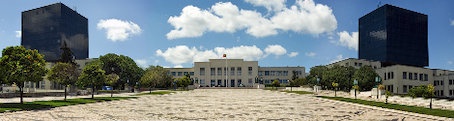
\includegraphics[width=\textwidth]{Figures/tecnico-lisboa.jpg}
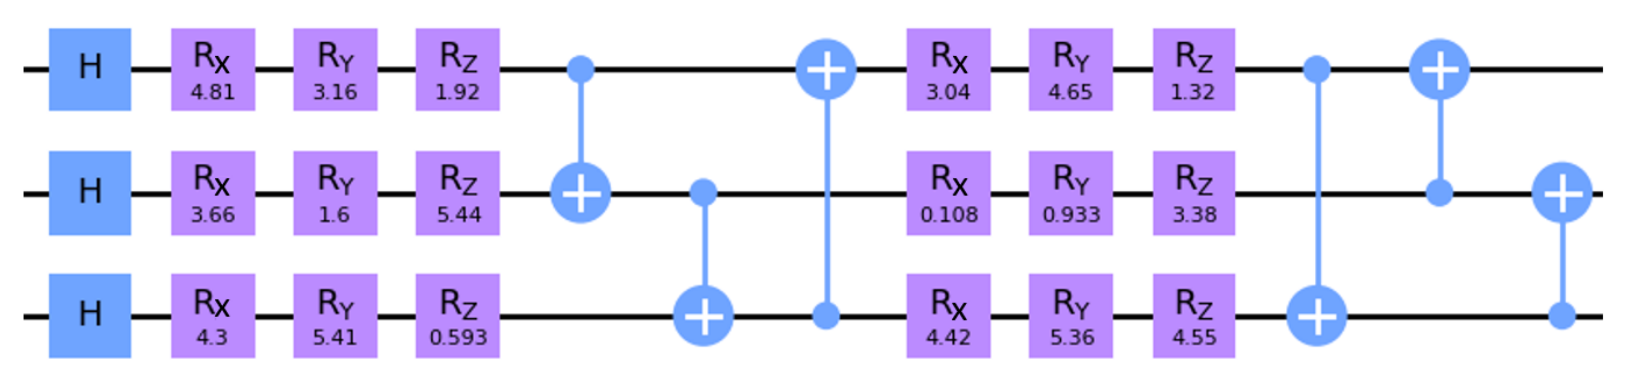
\includegraphics[width=\textwidth]{Figures/Diagrams/Strongly_Entangling_Layers.png}

% Title, author and degree
\vspace{1.0cm}
% {\FontLb Development of a new variational quantum algorithm for MaxCut: QAOA and QEMC hybrid algorithm} \\ % <<<<< EDIT TITLE. Old title.
{\FontLb Novel Variational Quantum Algorithms for MaxCut} \\ % <<<<< EDIT TITLE. New title.

% Alternative title: "A Framework for Variational Quantum Algorithms for MaxCut".

%\vspace{0.2cm}
%{\FontMn Subtitle (optional)} \\
%\vspace{1.9cm}
\vspace{2.6cm}
{\FontMb Afonso Sequeira Azenha} \\ % <<<<< EDIT NAME
\vspace{2.0cm}
{\FontSn \coverThesis} \\
\vspace{0.3cm}
{\FontLb Engineering Physics} \\ % <<<<< EDIT COURSE
\vspace{1.0cm}
{\FontSn %
\begin{tabular}{ll}
 \coverSupervisors: & Prof. Yasser Rashid Revez Omar \\ % <<<<< EDIT NAME
                    & Prof. João Carlos Carvalho de Sá Seixas    % <<<<< EDIT NAME
\end{tabular} } \\
\vspace{1.0cm}
{\FontMb \coverExaminationCommittee} \\
\vspace{0.3cm}
{\FontSn %
\begin{tabular}{c}
\coverChairperson:     Prof. Full Name 1  \\ % <<<<< EDIT NAME
\coverSupervisor:      Prof. Full Name 2  \\ % <<<<< EDIT NAME
\coverMemberCommittee: Prof. Full Name 3     % <<<<< EDIT NAME
\end{tabular} } \\
\vspace{1.5cm}
{\FontMb June 2024} \\ % <<<<< EDIT DATE (corresponds to date of oral examination)
%
\end{center}
